\section*{Formulation of the problem}\label{sec:approach}

The main challenge of applying quantum annealing to a real-world problem is in formulating the problem as Quadratic Unconstrained Binary Optimization (QUBO), i.e.\ a quadratic real-valued polynomial over Boolean-valued variables.
%
Specifically, we are focusing on the problem of minimizing the total delay of a set of flights (each consisting of an origin, destination, and departure time).
More precisely, we are given the wind-optimal trajectories for every flight, and wish to choose a set of modifications of these trajectories so that they a) do not conflict with each other, and b) minimize the sum of the delays of the flights at their destinations, relative to the wind-optimal trajectories.
%
To do so, we first had to parameterize the trajectory modifications in such a way that a) the parameterizations could be encoded in Boolean-valued variables, and b) the constraints and cost function (total delay) could be expressed as quadratic polynomial over those bits.
The modifications to the trajectories that we consider are of two types. 
First, we consider origination delays, in which the departure of the flight from its origin is simply delayed, and its trajectory translated in time only. 
Second, we consider avoidance maneuvers, in which flights may briefly change course in order to avoid conflicts with others;
a maneuver is local, and can only change the subsequent part of the trajectory by pushing it forward in time.

Given the set of wind-optimal trajectories, we refer to the points in space that more than one trajectory crosses at some time ``spatial conflicts''.
These serve as a starting point in that they allow us to discretely identify potential conflicts.
This allows us to parameterize the modified trajectories by the times at which every flight arrives at its potential conflicts.
Let let $t_{i,k}$ be the variable indicating the time at which flight $i$ gets to potential conflict $k$, and let $t_{i,k}^*$ be the wind-optimal value.
The difference between them $D_{i,k} = t_{i,k} - t^*_{i,k}$ is the accumulation of delays that flight $i$ encounters before conflict $i$.
Let $d_{i,k}$ be the variable indicating the delay added to flight $i$ at potential conflict $k$.
Then the delay can be written $D_{i,k} = d_i + \sum_{k' \in P_{i,k}} d_{i,k}$, where $d_i$ is the origination delay and $P_{i,k}$ is the set of potential conflicts that flight $i$ encounters prior to $k$.

Since the state-of-art quantum hardware has a limited amount of physical resources, we cannot take trace of all the possible
spatial conflicts. To overcome this limitation, we introduce the concept of actual conflicts, namely all those conflicts which occurs
within a specific time window $\theta$, i.e. $|t_{i,k} - t_{j,k}| \leq \theta$ for two flights $i$ and $j$ at potential conflict $k$.
This type of penalties can be done by encoding each time $t_{i,k} = \sum_{\alpha} \alpha t_{i,k,\alpha}$ using bits indicating its value from a discrete set $\{\alpha\}$, and adding the penalty term $\sum_{|\alpha - \beta| < \theta} t_{i,k,\alpha} t_{j,k,\beta}$.
We are currently exploring the relative advantages of encoding the trajectories using the absolute times $\{t_{i,k}\}$ or the relative delays $\{d_{i,k}\}$ (both lead to qualitatively similar resource requirements), as well as different ways of encoding the potential maneuvers, especially when multiple flights potentially conflict at the same point in space and time.

\begin{figure}
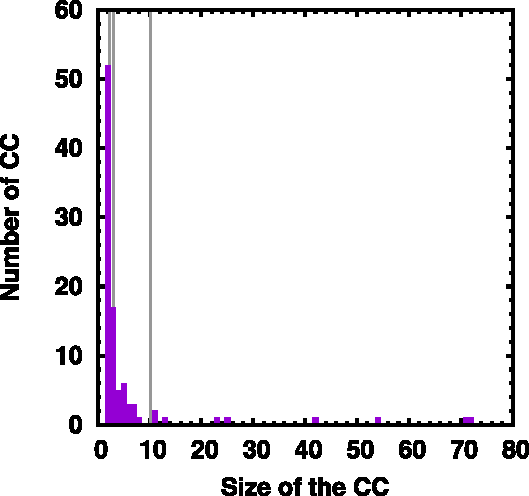
\includegraphics[scale=0.9]{images/cc_hist_mindist030_mintime060.pdf}
\end{figure}


\section*{Departure delay model on DW2X}

bla bla